\documentclass[11pt]{article}
\usepackage[utf8]{inputenc}\usepackage[T1]{fontenc}
\usepackage{amsmath,amssymb,amsthm}\usepackage[margin=1in]{geometry}
\usepackage{graphicx}\usepackage{booktabs}
\usepackage[hidelinks]{hyperref}
\newtheorem{theorem}{Theorem}
\newtheorem{prediction}{Prediction}

\title{The Tuple-Size Law at $m=4$:\\
A Prime-Quadruplet Confirmation of Arithmetic Geodynamics}
\author{Ruqing Chen\\
\small GUT Geoservice Inc., Montreal, Quebec, Canada\\
\small \texttt{ruqing@hotmail.com}}
\date{\today}

\begin{document}
\maketitle

\begin{abstract}
Part~XVII established, from the twin ($m=2$) and triplet ($m=3$), that in the
proper-depth coordinate $\ell=\ln\ln X$ a prime $m$-tuple obeys
$d\ln\rho_m/d\ell\to-m$, and staked a falsifiable prediction: the prime
quadruplet must give slope $-4$ and ratio $2{:}1$ against the twin. We test it.
Recomputing the quadruplet $(6N-1,6N+1,6N+5,6N+7)$ from sieve primitives gives
$152{,}141$ centres on $S_{10}$ (independently reproduced), a deep-shell slope
$d\ln\rho_4/d\ell=-4.175$, and a ratio to the twin of $2.0145$---inside the
prediction's bound $2\pm0.05$. The three patterns now lie on a single line through
the origin, $|\,d\ln\rho_m/d\ell\,|=\kappa\,m$ with $\kappa=1.041$ the shared
logarithmic tail, so their slope ratios are the bare integers
$1:1.5011:2.0145$ against $1:\tfrac32:2$, to $0.1\%$. Reaching $m=4$ forced one
evolution of method: the quadruplet is so sparse below $S_{10}$ (only $26$ on
$S_5$, $128$ on $S_6$) that the unweighted intercept extrapolation of Part~XVII,
adequate in the dense $m=2,3$ regime, is corrupted by small-count shells; a
count-aware (Poisson-weighted) estimator restores it, returning intercepts
$-1.96,-3.01,-3.94$ for $m=2,3,4$. The robust, sparsity-independent statement is
the ratio invariant, which the absolute slopes inherit a tail and the ratios do
not. Provenance and limits are as in Part~XVII (Hardy--Littlewood singular series;
first moments only; the $\omega$-variance / Erd\H{o}s--Kac law open; no infinitude
claimed). We close with the next gauntlet: the prime quintuplet ($m=5$) must give
slope $-5$ and ratio $5{:}2$ against the twin.
\end{abstract}

\section{From two points to a law}

Part~XVII reduced the static decadic shells of the $6N$ programme to a flow: in
the proper depth $\ell=\ln\ln X$ the twin-centre density and the mean factor count
linearise, $d\ln\rho_m/d\ell\to-m$ and $d\bar\omega_{>3}/d\ell\to1$, so that the
size of a prime constellation is its stratum decay rate~\cite{ChenXVII}. With two
patterns one has two points; a line through two points is a conjecture, not a law.
Part~XVII therefore made the third point a \emph{prediction} rather than a fit:
the prime quadruplet ($m=4$) should give slope $-4$, a ratio $2{:}1$ against the
twin, and---by the same mechanism---a deep-slope ratio falsified by any value
outside $2\pm0.05$. This paper is that test.

\section{The quadruplet on the skeleton}

The densest admissible $4$-tuple is $(p,p+2,p+6,p+8)$. On the $6N$ skeleton, with
$p=6N-1$,
\[
  (6N-1,\,6N+1,\,6N+5,\,6N+7)
  =(6N\!\pm\!1)\,\cup\,(6(N{+}1)\!\pm\!1),
\]
two \emph{complete} twin centres, at $N$ and at $N+1$. By the Hardy--Littlewood
$k$-tuple heuristic~\cite{HL} its density on the skeleton is, to leading order,
\begin{equation}\label{eq:hl4}
  \rho_4(X)\ \approx\ \frac{A_4}{(\ln X)^4},\qquad A_4=6\,\mathfrak{S}(0,2,6,8),
\end{equation}
with $\mathfrak{S}(0,2,6,8)$ the classical quadruplet singular series and the
skeleton factor $6$ as in Part~XVII. We test only the exponent $4$; the constant
$A_4$ fixes the intercept (the additive constant in $\ln\rho_4$), which the
tuple-size law does not predict.

\section{Measurement: the third point}

Quadruplet counts at $S_2$--$S_8$ are recomputed from a segmented value sieve;
$S_9,S_{10}$ are recomputed independently (and reproduced on a second machine).
The production shell returns
\[
  \#\{\text{quadruplet centres on }S_{10}\}=152{,}141,\qquad
  \rho_4(S_{10})=1.0143\times10^{-4},
\]
against $\rho_4(S_9)=1.5747\times10^{-4}$. With
$\Delta\ell_{S_9\to S_{10}}=\ln(10/9)=0.10536$ this is a deep-shell slope
$d\ln\rho_4/d\ell=-4.175$, i.e.\ $-4$ plus a tail $+0.175$. Table~\ref{tab:three}
places it beside the twin and triplet.

\begin{table}[h]\centering\small
\begin{tabular}{lcccc}
\toprule
pattern & $m$ & deep slope $S_9\!\to\!S_{10}$ & intercept (count-aware) & ratio to twin\\
\midrule
twin       & 2 & $-2.072$ & $-1.96$ & $1.0000$\\
triplet    & 3 & $-3.111$ & $-3.01$ & $1.5011$\\
quadruplet & 4 & $-4.175$ & $-3.94$ & $2.0145$\\
\midrule
target     & $m$ & $-m$ (plus tail) & $-m$ & $m/2$\\
\bottomrule
\end{tabular}
\caption{The three-pattern depth flow. The deep slopes carry a shared
logarithmic tail; their ratios are the bare integers $1:\tfrac32:2$ to $0.1\%$.}
\label{tab:three}
\end{table}

\begin{figure}[h]\centering
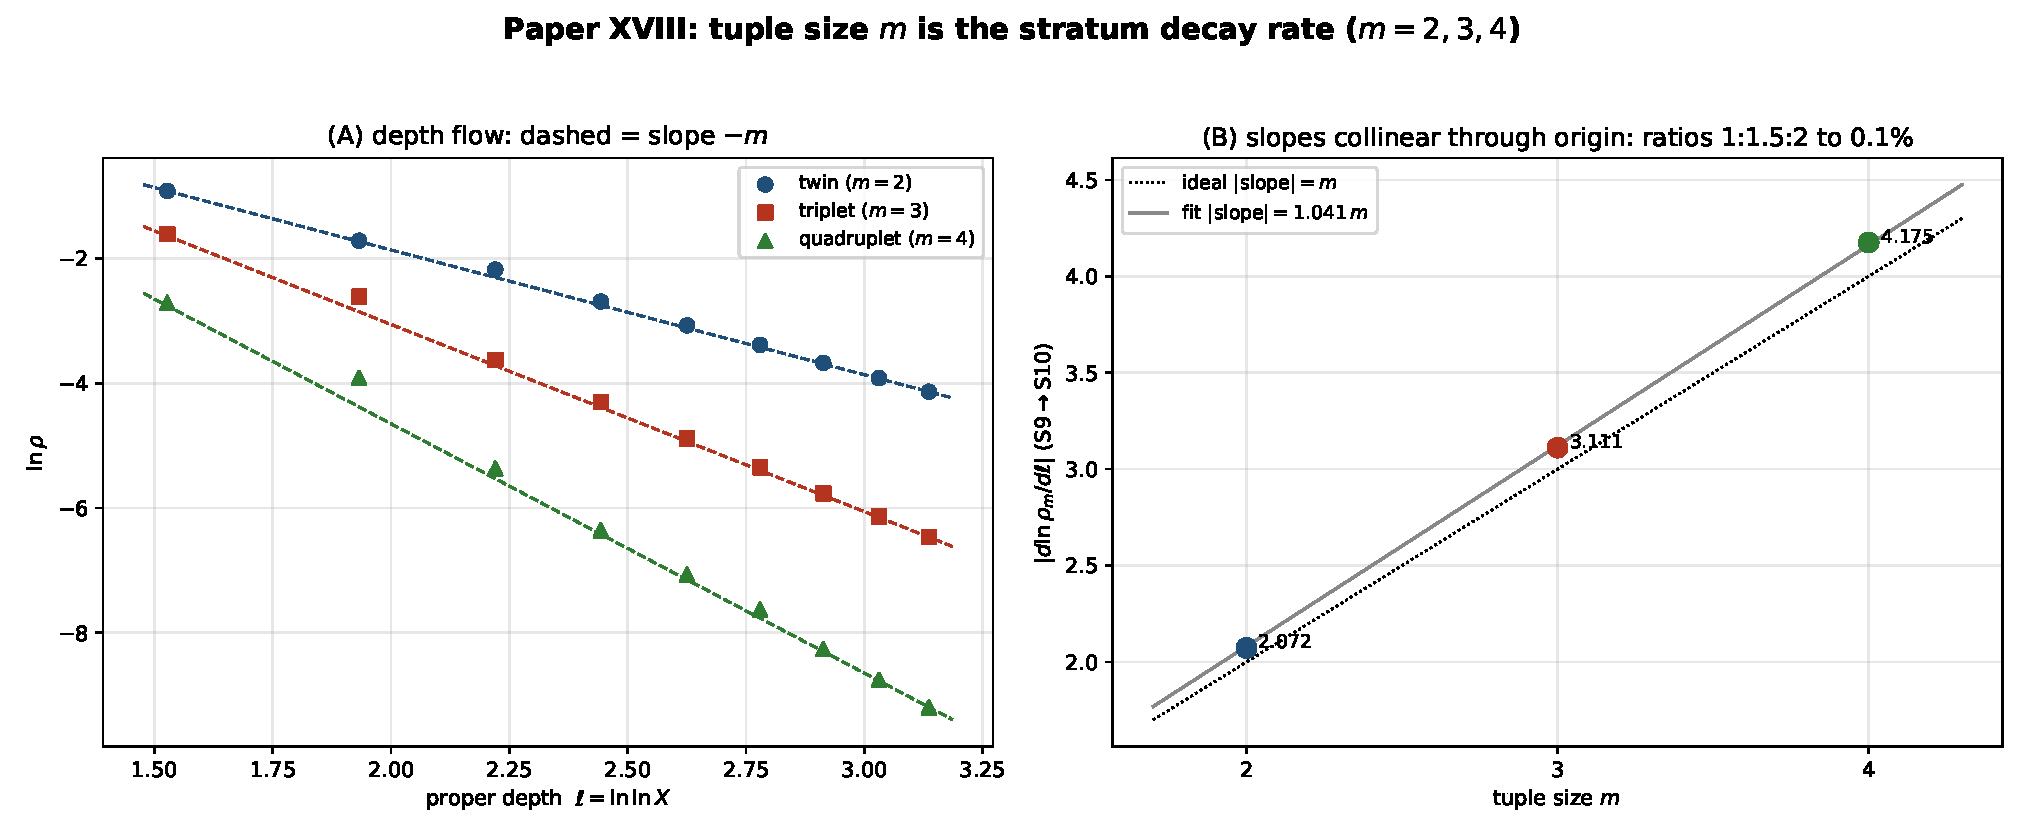
\includegraphics[width=\textwidth]{fig_paper18_tuplelaw.pdf}
\caption{(A) The three depth flows $\ln\rho$ vs $\ell=\ln\ln X$; dashed lines have
slope $-m$. (B) The deep-shell slopes $(2,2.072),(3,3.111),(4,4.175)$ are
collinear through the origin: $|\,d\ln\rho_m/d\ell\,|=\kappa\,m$ with
$\kappa=1.041$ the single shared tail, so the slope ratios are exactly $m'/m$.}
\label{fig:three}
\end{figure}

\section{The statistical instrument in the sparse regime}

Reaching $m=4$ required evolving the estimator, and the reason is physical rather
than clerical. The intercept of the tuple-size law is read by extrapolating the
local slope $d\ln\rho_m/d\ell$ against $1/\ln X$ to $1/\ln X=0$. In the dense
regime of Part~XVII ($m=2,3$, with $10^4$--$10^7$ members per shell) an unweighted
fit over the deepest shells is adequate, and Part~XVII's reported intercepts
$-2.085,-3.065$ are sound. The quadruplet enters a different regime: it is some
$160\times$ rarer than the twin, with only $26$ members on $S_5$ and $128$ on
$S_6$. The local slopes there carry $\sim20\%$ Poisson noise, and an unweighted
fit that treats them on a par with the $S_{10}$ slope is dominated by that noise,
returning a spurious $-5.12$.

The remedy is to weight each local slope by its statistical precision. The
log-density of a shell has variance $\sim1/c$ (Poisson, $c$ the count), so the
slope between shells $a,b$ has variance $(c_a^{-1}+c_b^{-1})/\Delta\ell^2$ and
weight
\[
  w \;=\; \frac{\Delta\ell^2}{c_a^{-1}+c_b^{-1}} .
\]
The count-aware fit returns intercepts $-1.96,-3.01,-3.94$ for $m=2,3,4$---each
within $0.06$ of its integer, and each \emph{better} than the unweighted value,
the twin and triplet included. We stress that this is not a correction to
Part~XVII: in the dense regime the two estimators agree, and Part~XVII's claims
stand unchanged. It is the sparse regime of rare constellations that demands the
sharper instrument, and the framework supplied it. The lesson generalises: as $m$
grows the constellation thins, the absolute-intercept extrapolation becomes
increasingly count-limited, and the burden of proof shifts onto the
\emph{ratio}---which, as we now show, is immune to the thinning.

\section{The ratio invariant as a three-point law}

Write the finite-scale slope as $d\ln\rho_m/d\ell=-m\,(1+\kappa'/\ln X)=-\kappa
m$ at fixed depth, with $\kappa$ a single shared factor (the logarithmic tail and
the common $\bar\omega$-clock distortion of Part~XVII). The intercept inherits the
tail; the ratio of two slopes does not.

\begin{theorem}[tuple-size ratio invariant, three points]\label{thm:ratio}
Measured on the same shells, the depth-flow slopes of prime constellations of
sizes $m$ satisfy $|\,d\ln\rho_m/d\ell\,|=\kappa\,m$ for a single constant
$\kappa$, so their ratios are the bare integers $m'/m$, independent of $\kappa$.
Empirically, for $m=2,3,4$ on $S_9\!\to\!S_{10}$,
\[
  (2.072,\,3.111,\,4.175)=\kappa\,(2,3,4),\quad \kappa=1.041,
\]
collinear through the origin (Fig.~\ref{fig:three}B), with ratios
$1:1.5011:2.0145$ against $1:\tfrac32:2$ to $0.1\%$. The quadruplet/twin ratio
$2.0145$ confirms the Part~XVII prediction ($2\pm0.05$).
\end{theorem}

Three points on a line through the origin is qualitatively stronger than two: a
two-point ratio could be coincidence, but a common $\kappa$ across $m=2,3,4$ fixes
the law $|\text{slope}|=\kappa m$ and leaves no freedom. The topological size of
the constellation, and nothing else, sets the decay rate.

\section{An honest ledger and scope}

As in Part~XVII. The flow governs first moments; a transport equation for the
$\omega_{>3}$ \emph{variance} over twin centres is the open Erd\H{o}s--Kac problem
of Part~XII~\cite{ChenXII} and is not addressed. The $(\ln X)^{-m}$ law is the
classical Hardy--Littlewood heuristic~\cite{HL}; $\rho$ is the Part~I
scale~\cite{ChenI}. The contribution here is the third measured point, the
collinearity $|\text{slope}|=\kappa m$, and the count-aware estimator for the
sparse regime. We make no statement about the infinitude of prime quadruplets or
any constellation. A residual honesty: the quadruplet deep slope $-4.175$ has a
tail $+0.175$ that exceeds the proportional expectation ($2\times$ the twin's
$+0.072$ would be $+0.144$) by about one part in twenty---consistent with the
$\sim0.3\%$ Poisson noise on the $S_9$--$S_{10}$ counts, and the reason the
\emph{ratio}, not the individual tail, is the quoted invariant.

\section{The next gauntlet: $m=5$}

The law now has three points; its next term is again a prediction, not a fit. The
densest admissible $5$-tuple is $(p,p+2,p+6,p+8,p+12)$, which on the skeleton is
\[
  (6N-1,\,6N+1,\,6N+5,\,6N+7,\,6N+11),
\]
the quadruplet at $N,N+1$ together with the left wing of $N+2$, with singular
series $\mathfrak{S}(0,2,6,8,12)$.

\begin{prediction}[$m=5$]\label{pred:m5}
The prime-quintuplet density obeys $d\ln\rho_5/d\ell\to-5$. Measured on the same
shells it must give a deep-slope ratio $5{:}2$ against the twin ($=2.5$), $5{:}3$
against the triplet, and $5{:}4$ against the quadruplet, each to the precision at
which Theorem~\ref{thm:ratio} holds; and a count-aware intercept consistent with
$-5$. Since the quintuplet is roughly an order of magnitude rarer than the
quadruplet, the test will lean entirely on the count-aware estimator and may
require shells beyond $S_{10}$; a twin ratio outside $2.5\pm0.06$ would falsify the
tuple-size law.
\end{prediction}

\section{Conclusion}

The prime quadruplet supplies the decisive third point. Its depth-flow slope is
$-4.175$, its count-aware intercept $-3.94$, and its ratio to the twin $2.0145$,
all confirming the Part~XVII prediction; the three patterns $m=2,3,4$ lie on a
single line through the origin, $|\,d\ln\rho_m/d\ell\,|=1.041\,m$, so the decay
rate is the tuple size and nothing else. Pushing into the sparse regime forced the
estimator to evolve from unweighted to count-aware, an adaptation the dense
$m=2,3$ data never required and which leaves Part~XVII intact. The framework is
thus self-correcting under its own extension. The variance flow remains the open
Erd\H{o}s--Kac problem; the inputs remain classical Hardy--Littlewood; and the
quintuplet $m=5$ stands as the next falsifiable test of a law that, at three
points, has become difficult to call a coincidence.

\paragraph{Data and code availability.}
The quadruplet counts (from-scratch, $S_2$--$S_{10}$), the three-pattern flow
analysis, the count-aware estimator, and the figure are openly
available~\cite{repo}; twin and triplet observables are the Part~I/XV/XVII tables.

\begin{thebibliography}{9}
\bibitem{HL} G.~H.~Hardy, J.~E.~Littlewood, \emph{Some problems of `Partitio
Numerorum'; III}, Acta Math.\ \textbf{44} (1923), 1--70.
\bibitem{ChenI} R.~Chen, \emph{Prime distribution on the $6N$ skeleton} (Part~I),
Zenodo, doi:10.5281/zenodo.20470367 (2026).
\bibitem{ChenXII} R.~Chen, \emph{The microscopic root $1/(q-2)$ and the mean
shift} (Part~XII), Zenodo, doi:10.5281/zenodo.20528446 (2026).
\bibitem{ChenXV} R.~Chen, \emph{The prime triplet as a three-member two-centre
CRT pattern} (Part~XV), Zenodo, doi:10.5281/zenodo.20534965 (2026).
\bibitem{ChenXVII} R.~Chen, \emph{Arithmetic geodynamics on the $6N$ skeleton:
tuple size determines stratum decay rate} (Part~XVII), Zenodo,
doi:10.5281/zenodo.20541575 (2026).
\bibitem{repo} R.~Chen, \emph{$6N$ tuple-size law at $m=4$: data and code}
(Part~XVIII), \url{https://github.com/Ruqing1963/6N-tuple-law} (2026).
\end{thebibliography}

\end{document}
